% This is LLNCS.DEM the demonstration file of
% the LaTeX macro package from Springer-Verlag
% for Lecture Notes in Computer Science,
% version 2.4 for LaTeX2e as of 16. April 2010
%
\documentclass{llncs}
%
\usepackage{graphicx}
\usepackage{amsmath}

%\usepackage{makeidx}  % allows for indexgeneration
%
\begin{document}
%
\frontmatter          % for the preliminaries
%
\pagestyle{headings}  % switches on printing of running heads
\addtocmark{Non-Parametric Transformation Networks} % additional mark in the TOC
%
\mainmatter              % start of the contributions
%
\title{Non-Parametric Transformation Networks}
%
\titlerunning{Non-Parametric Transformation Networks}  % abbreviated title (for running head)
%  
%
\author{Daniel Biskup and Catherine Capellen}
%
\authorrunning{Daniel Biskup and Catherine Capellen} % abbreviated author list (for running head)
%
%%%% list of authors for the TOC (use if author list has to be modified)
\tocauthor{Daniel Biskup and Catherine Capellen}
%
\institute{University of Bonn}

\maketitle              % typeset the title of the contribution

\begin{abstract}
The abstract 
\end{abstract}
%

\section{Introduction}
CNNs are state of the art in image recognition tasks [FIND CITE]. Certain kind of transformations on these images will not affect the class of the depicted object. 
Examples for this are small translations, rotations or perspective transforms. Other kind of translations might change the object class, for example if you rotate the image of the number 6, it will look like a 9. 
Using augmented data in training as well as choices in the architecture of CNNs as pooling layers aim to improve the robustness of CNNs to specific transformations. 
Pooling is a method that is usually performed spatially, meaning that the 

GENERAL TOPIC: Object recognition, CNNs, POOLING, PTN/NPTN, Paper results (SHORT) 
TASK
ROTNET TASK

\section{Networks Architectures ( aka Methods)}
The kinds of networks this report is concerned with are Convolutional Neueral Networks (CNNs), Non-Parametric Transformation Networks (NPTNs), a custom network architecture we call RotNets.

\subsection{Convolutional Neueral Networks}
NPTNs can be seen as a generalization of CNNs. For that reason we will briefly discuss CNNs.
\subsubsection{Convolution}
As the name suggests, NPTSn make heavy use of the Convolution Operation. Convolutions, as illustraded in Figure \ref{fig:conv}, calculate the weighted sum over a sub region of an input image in order to calculate the pixel-values of the output. The weights used for calculation the weighted sum are given by a matrix called filter or Kernel. Naturally different Kernels produce different results. In Computer Vision they are used to detect different kinds patterns. Thus one kernel might respond to vertical edges, another  one to horizontal edges and yet another one to yet another pattern. While kernels traditionally got designed by experts in Computer Vision, whithin CNNs they are expected to be learned by the network.

\begin{figure}
	\begin{center}
		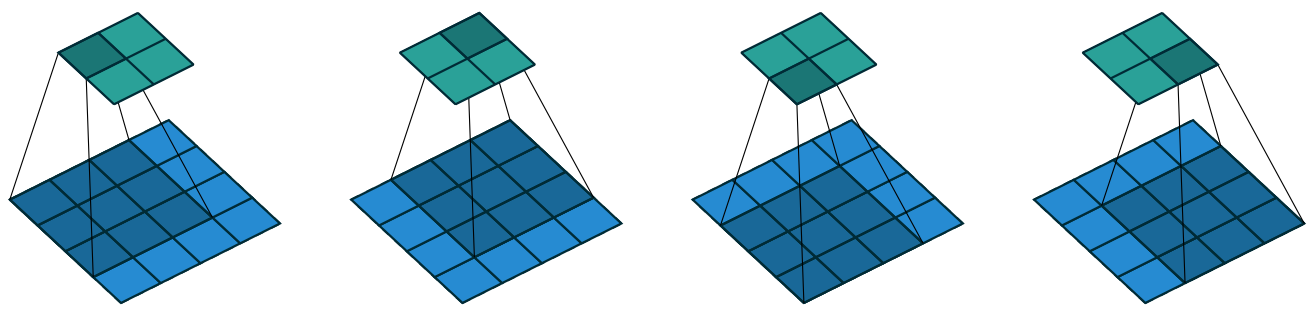
\includegraphics[width=\textwidth]{result_images/Conv.png}
		\caption{Convolving a 3 × 3 kernel over a 4 × 4 input using unit strides}
		\label{fig:conv}
	\end{center}
\end{figure}

\subsubsection{Spatial Max Pooling}
Another important operation used in CNNs is Max Pooling.
Each neuron in the max pooling layer takes into account only a subregion of the previous
layers output and takes the maximum value of it to be it's output. By doing this they make the network invariant to small translations. Max pooling is illustrated in Figure \ref{fig:maxpooling}.

\begin{figure}
	\begin{center}
		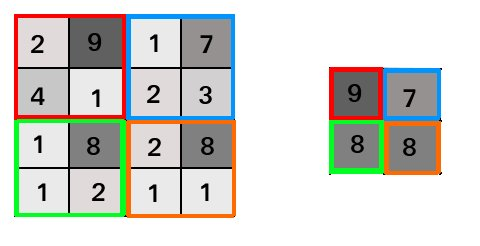
\includegraphics[width=0.40\textwidth]{result_images/maxpooling.jpg}
		\caption{Max Pooling in CNNs}
		\label{fig:maxpooling}
	\end{center}
\end{figure}

\subsection{Parametric and Non-Parametric Transformation Networks}
\begin{itemize}
  \item	mathmotivation
  \item Architecture
  \item How they are a generalization of CNNs
\end{itemize}

Paramateric Transformation Networks (PTNs) and Non-Parametric Transformation Networks, as introduced in \cite{NPTN} try to add more tranformation invariance to CNNs. For this Max Pooling over layers is used. 
Where a CNN has one filter, PTNs and NPTNs have $|G|$ filters and a pixel wise max pooling operation is performed over the filters, such that for each pixel the strongest result of the convolution with a filter is used. [IMAGE]

For the PTNs these $|G|$ filters are transformations of a base filter with weights $w$. The transformations belong to a (unitary) group of transformations and are learned simultaniously to $w$ for each of the different $w$. [MAYBE use TN nodes for explanation?]



\subsection{RotNets}
Rotation Networks (RotNets) were our idea for the additional task of designing a network that is due to its structure invariant to rotations. 
The idea is based on the same structure as PTNs (and NPTNs), just that the group of transformations is fixed to be rotations. Therefore there exists one set of weights $w$, which is learned for each $|G|$ transformations and this weights are rotated into the new kernels. 
[ALPHA]

\section{Implementation in with PyTorch}
Because the authors of the paper in NPTNs state, that they used PyTorch for their experiments, and because PyTorch is widely accepted and adopted within the scientific community, we decided to base our experiments on PyTorch as well.
To be able to reproduce the experiments performed in the paper, we had to implement the NPTN layer. To see if our approach, the RotNet, would perform well we had to implement it as well.

When implementing new network architectures in PyTorch it's crucial to specify which values AutoGrad should view as parameters of the network in order for it to be able to apply backpropagation algorithm to the network. Furthermore you need to take care, that all calculations and operations performed in the forward path are differentiable by AutoGrad.
\subsection{The NPTN Layer}
%TODO Add NPTN graphics!
Our implementation follows the description given in the NPTN paper.
Lets say we have M inputs and want N outputs while using a set of G different filters for each path from input to output.
Just as for CNNs, all filters we use during convolution are also parameters that are expected to be learned by the network.
For this reason we can perform the convolutions by using an instance of the nn.Conv2d layer which will automatically initialize the filters and also register them as learn able parameters. This way, by using nn.Conv2d we don't need to worry about AutoGrad and differentiability of parameters ourself.

In it's constructor we specify it to have M inputs and M*N*G outputs. The important implementation detail here is, that we need to set the groups option to M, which causes Conv2d to use a filter bank of N*G filters per input.

%TODO DEL USE SPACE NEEDED__ 
Usually the output value of the nn.Conv2d layer with input size $(N, C_{in}, H, W)$ and output $(N, C_{out}, H_{out}, W_{out})$ can be precisely described as:
\begin{equation*}
\text{out}(N_i, C_{out_j}) = \text{bias}(C_{out_j}) +
\sum_{k = 0}^{C_{in} - 1} \text{weight}(C_{out_j}, k) \star \text{input}(N_i, k)
\end{equation*}
but since setting groups to M causes nn.Conv2d to operate as if there are M conv layers side by side, each seeing one input channel and producing N*G output channels, $C_{in} = 1$, which means, that there will be no weighted sum since only one convolution will be calculated per output.
%TODO __DEL USE SPACE NEEDED

After calling the convolution, we have a tensor with N consecutive packs of G layers produced by the same input. But we want need that G layers of input 1 are followed by G layers of input 2 and so on. This can be archived by a simple permutation, which we decided to defer until after the max pooling across channels. We will come back to this permutation later.

Next we use nn.MaxPool3d with stride 1 and kernel size (G,1,1). Note, that this does not resemble spatial max pooling as is commonly used in CNNs, but rather the pixel wise maximum of G consecutive layers.

Following this, to perform the aforementioned permutation, we defined a matrix of numbers from 0 to the number of layers left in the tensor, permuted it, and then indexed the tensor with it. Note, that this is valid, because indexing tensors is tracked by AutoGrad.
%TODO Maybe add: Permutation with matrix as formula.

This is followed by the Average Pooling across layers, which is common to CNNs and actually replaces the weighted sum operation in the formula of $\text{out}(N_i, C_{out_j})$ above. This can be archived by using nn.AvgPool3d.

\subsection{The RotNet Layer}
%TODO BORIS
DETERMINATION OF NETWORK DIMENSION (48,16): EQUAL AMOUNT
OF PARAMETERS
ROTNET: GRIDSAMPLER, DIFFERENTIABLE
(DIMENSION DING)
NPTN IMPLEMENTATION

\subsubsection{The convolution}
Within the implementation of the NPTN layer we were able to use an instantiation of the nn.Conv2d layer, because we had to learn each kernel we used individually, i.e every kernel used for convolution was also a parameter of the network.\\
For the RotNet layer on the other hand, we need to use the nn.functional.conv2d function which expacts as argument the kernels we want to use, while inside the definition of the NPTN layers class we only "mark" the unrotated kernels as parameters by calling "" on them.

\subsubsection{GRIDSAMPLER, DIFFERENTIABLE}

\subsection{Multi Layer Networks}
\subsubsection{Determining the size of individual network layers}
Once the network layers needed are defined, and before useful experiments can be run, one has to stack multiple of them on top of each other to build multi layered networks.
Unfortunately the NPTN paper didn't specify the size of each layer precisely enough, which forced us to guess and try different values.

The idea is to keep the number of parameters in the networks we want to compare roughly equivalent to allow comparisons between the different architectures performances.

%TODO Fill in more detail here...

\subsubsection{Input size to fully connected layer}
Can be calculated dynamically.
\subsubsection{YAML files for Experiment setup}

4 EXPERIMENTS
- DESIGN (WHAT WAS IN PAPER AND WHAT WASN'T)



\section{Experiments and Results}	
In the following we will present three experiments from the paper that we tried to reproduce and tried to mimic as closely as possible. 
All the experiments use a two-layered or three-layered structure which include either a NPTN layer, a Convolutional layer or a RotNet layer in each layer. The structure for the two-layered network is shown in Figure \ref{pic:net_structure}. The last softmax layer is not described in the paper, but was added by us [WHY softmax, because it's standard]. 

\begin{figure}
	\begin{center}
	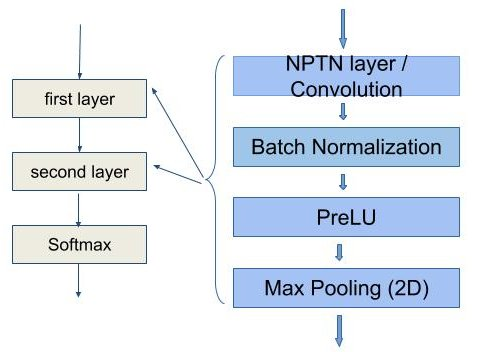
\includegraphics[scale=0.35]{result_images/network_structure.jpg}
	\caption{Structure of a two layered network.}
	\label{pic:network_structure}
	\end{center}
\end{figure}

\subsection{Experiments on CIFAR10}
The first experiment used the CIFAR10 dataset [CITE]. A CNN and several NPTNs with different values for G are tested. The dimension of the NPTNs is changed for the different values of G such that all networks have the same amount of filters.
The paper describes in detail the setup of the experiments regarding learning rate, data preprocessing and network dimensions. However other important information as filter size and loss function is missing. 
For the filtersize we used 5, since in the other experiments, the paper mentions  filtersizes of 3,5 or 7 and 5 often shows the best performance for the NPTNs. 
In Figure \ref{pic:first_experiment} we show the results from the paper next to our experimental results. For the loss function we chose Negative Log Likelihood Loss (NLLL) [WHY]. 
However we did not get any comparable loss values as in the paper. Comparing the loss values of the networks to each other, in the paper, all NPTNs perform better than the CNN. In our results, only one of the NPTNs performs better.
Since we are not sure if the loss used in the paper is the same, we also calculated the accuracy of the networks. The values are consistent with the loss for this experiment, so for each network if the loss is lower, then the accuracy is higher compared to other networks.

\begin{figure}
	\begin{center}
	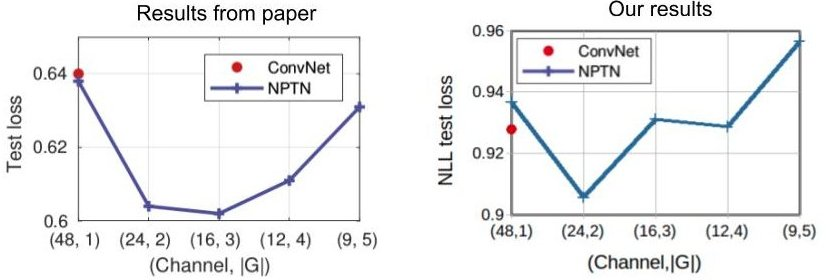
\includegraphics[scale=0.35]{result_images/experiment1.jpg}
	\caption{The first experiment}
	\label{pic:first_experiment}
	\end{center}
\end{figure}

TRAIN vs TEST ERROR?

\section{Rotation Experiments on MNIST}
The second experiment from the paper compares a CNN and several NPTNs. Again the dimensions are chosen in a way that matches the values in the paper and leads to the same amount of filters for all networks. 
This experiment uses the MNIST dataset [CITE] where all images from training and test set were randomly rotated up to a certain degree. 
The paper shows the results from various maximal rotation degrees. we picked the two strongest rotations, since the performance difference between NPTNs and CNNs was the biggest there and performed our own experiments, adding also RotNets for comparison.
The Paper did specify the data preprocessing in detail, but didn't give new instructions for learning rate, so we kept the same experiment setup as in the first experiment.
The results from our experiments are shown in Figure \ref{pic:second_experiment}. [TODO: new graphic?]


\section{Three-layered-networks}
This experiment from the paper compares three-layered NPTNs and CNNs of the CIFAR10 dataset [CITE]. 
The network dimensions are not described well and the paper states that the amount of parameters for those networks is similar, but not exactly the same as in the previous experiments. 
Therefore we determined possible dimensions for the amount of channels in the NPTNs and CNNs. 
Again no new learning rate was given for this experiment, so we initially tried with the same experimental setup as in the first two experiments, but using this and the dimensions that seemed likely from the paper led the networks to overfit greatly and the loss values did not improve. 
Therefore we reduced the amount of parameters and the learning rate and achieved a result, which had less generalization error. 
Different than in the first two experiments accuracy and loss are not consistent anymore. While the loss starts getting worse after some iteration, the accuracy stays approximately stable and we therefore used the accuracy to compare the networks.
[TODO show results]

\section{Experiments for RotNet}
The final experiment was designed by us to see if RotNet was able to perform one of the ideas behind its design: the ability to be invariant to rotations without learning them. For this we copied the setup of the MNIST rotation experiment with the difference, that this time we only rotated the test set. The results are shown in Figure [FIG]. 


\section{Discussion and further work}
TRAIN vs TEST ERROR?
CONCLUSION: PAPER IS NOT REPRODUCABLE NPTNs FROM THIS
EXPERIMENTS NOT BETTER ( ROTNET BAD

WHY WE THINK NPTNS ARE LESS POWERFULL WHY ROTNETS ARE
WORSE THAN NPTNs WHY IT IS MAYBE NOT A GOOD IDEA TO RO-
TATE EARLY FILTERs

\section{What we learned}
Dealing with tensor dimensions.
Implement networks architectures using PyTorch.

%
% ---- Bibliography ----
%
\begin{thebibliography}{}
%
\bibitem[1]{NPTN}
Pal, D. K., \& Savvides, M. (2018). Non-Parametric Transformation Networks. arXiv preprint arXiv:1801.04520.


%TODO References to add:
% Websites
% - PyTorch Documentation: http://pytorch.org/docs/0.3.1/
%
% Papers
% - NPTN paper: https://arxiv.org/abs/1801.04520v3
%
% Figures
%   Convolution: https://arxiv.org/abs/1603.07285v2


\end{thebibliography}
%\clearpage
%\addtocmark[2]{Author Index} % additional numbered TOC entry
%\renewcommand{\indexname}{Author Index}
%\printindex
%\clearpage
%\addtocmark[2]{Subject Index} % additional numbered TOC entry
%\markboth{Subject Index}{Subject Index}
%\renewcommand{\indexname}{Subject Index}
%%                                                           clmomu01.ind
%-----------------------------------------------------------------------
% CLMoMu01 1.0: LaTeX style files for books
% Sample index file for User's guide
% (c) Springer-Verlag HD
%-----------------------------------------------------------------------
\begin{theindex}
\item Absorption\idxquad 327
\item Absorption of radiation \idxquad 289--292,\, 299,\,300
\item Actinides \idxquad 244
\item Aharonov-Bohm effect\idxquad 142--146
\item Angular momentum\idxquad 101--112
\subitem algebraic treatment\idxquad 391--396
\item Angular momentum addition\idxquad 185--193
\item Angular momentum commutation relations\idxquad 101
\item Angular momentum quantization\idxquad 9--10,\,104--106
\item Angular momentum states\idxquad 107,\,321,\,391--396
\item Antiquark\idxquad 83
\item $\alpha$-rays\idxquad 101--103
\item Atomic theory\idxquad 8--10,\,219--249,\,327
\item Average value\newline ({\it see also\/} Expectation value)
15--16,\,25,\,34,\,37,\,357
\indexspace
\item Baker-Hausdorff formula\idxquad 23
\item Balmer formula\idxquad 8
\item Balmer series\idxquad 125
\item Baryon\idxquad 220,\,224
\item Basis\idxquad 98
\item Basis system\idxquad 164,\,376
\item Bell inequality\idxquad 379--381,\,382
\item Bessel functions\idxquad 201,\,313,\,337
\subitem spherical\idxquad 304--306,\, 309,\, 313--314,\,322
\item Bound state\idxquad 73--74,\,78--79,\,116--118,\,202,\, 267,\,
273,\,306,\,348,\,351
\item Boundary conditions\idxquad 59,\, 70
\item Bra\idxquad 159
\item Breit-Wigner formula\idxquad 80,\,84,\,332
\item Brillouin-Wigner perturbation theory\idxquad 203
\indexspace
\item Cathode rays\idxquad 8
\item Causality\idxquad 357--359
\item Center-of-mass frame\idxquad 232,\,274,\,338
\item Central potential\idxquad 113--135,\,303--314
\item Centrifugal potential\idxquad 115--116,\,323
\item Characteristic function\idxquad 33
\item Clebsch-Gordan coefficients\idxquad 191--193
\item Cold emission\idxquad 88
\item Combination principle, Ritz's\idxquad 124
\item Commutation relations\idxquad 27,\,44,\,353,\,391
\item Commutator\idxquad 21--22,\,27,\,44,\,344
\item Compatibility of measurements\idxquad 99
\item Complete orthonormal set\idxquad 31,\,40,\,160,\,360
\item Complete orthonormal system, {\it see}\newline
Complete orthonormal set
\item Complete set of observables, {\it see\/} Complete
set of operators
\indexspace
\item Eigenfunction\idxquad 34,\,46,\,344--346
\subitem radial\idxquad 321
\subsubitem calculation\idxquad 322--324
\item EPR argument\idxquad 377--378
\item Exchange term\idxquad 228,\,231,\,237,\,241,\,268,\,272
\indexspace
\item $f$-sum rule\idxquad 302
\item Fermi energy\idxquad 223
\indexspace
\item H$^+_2$ molecule\idxquad 26
\item Half-life\idxquad 65
\item Holzwarth energies\idxquad 68
\end{theindex}

\end{document}
